\chapter{Results}

In the end I had XXXX operational camera trap days, where XXX in the control group A, YYY in group B and ZZZ in group C. Pooled together, group B and C had MMM days with an additional white LED camera (flash = TRUE), and NNN days with only an IR camera (flash = FALSE).  %Present in table


Of all the detected species, the most common were roe deer(), red fox(), hare(), badger(), moose(), squirrel(), red deer() and European pine marten(). There were BBBBB photos of nothing, where ~9000 were time lapses (reconyx), the rest of them were continuing series, likely triggered by vegetation in front of the trigger (GGG events, HHH photoseries), or single events (CCC). 


\subsection{Number of pictures taken or whatnot}
\begin{table}

\caption{\label{tab:}Table with kable}
\centering
\begin{tabular}[t]{l|r|r|r|r|r}
\hline
  & A Control & B\ IR & B\ LED & C\ IR & C\ LED\\
\hline
elg & 128 & 78 & 90 & 75 & 57\\
\hline
grevling & 217 & 123 & 254 & 254 & 125\\
\hline
raadyr & 608 & 271 & 249 & 396 & 395\\
\hline
rev & 257 & 152 & 202 & 195 & 160\\
\hline
\end{tabular}
\end{table}

There were a peak number of photos taken between april and october, when excluding photos of "nothing" from the count. January and February are incomplete months, in both 2019 and 2020, and hence cannot be fairly compared to the other months in this barplot. %TODO Labels for total camera days per month


\section{Overlap analysis}

\begin{figure}
\centering
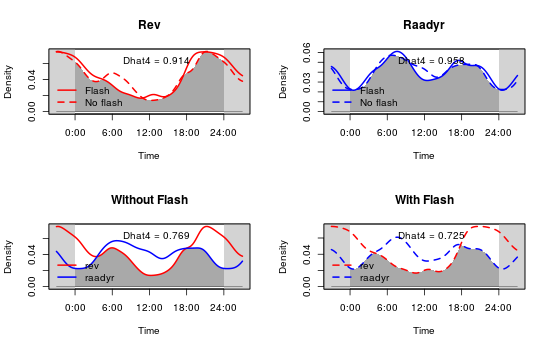
\includegraphics[scale=.7]{Rplot/overlap_rev_raa.png}
	\label{fig:overlap_rev_raa}
\end{figure}


For foxes, sites with only IR flash produced a more rugged curve than did the sites with a white LED flash.
Proportion of foxes at sites were markedly lower before sunrise, and then higher afterwards. 
Interestingly, there were more datapoints from the IR sites, which would usually produce smoother curves, by picking up less random variation. 
There is a resembling phenomenon happening in the evening twilight as well, right before the peak time of activity before midnight.

The Dhat4 calculation reveals a larger difference in overlap for foxes, than for roe deer, but this seems to mainly stem from the twilight hours.

% Table of Dhat4 scores for the most frequent species?

\section{Box plots}

%\begin{figure}
%\centering
%\includegraphics[scale=.7]{Rplot/box_abc_flash.png}
%	\label{fig:box_abc_flash}
%\end{figure}

There were no significant changes in frequencies of any of the most common species when a white LED was present compared to when it was absent. Perhaps a slight trend towards higher frequencies in the white LED periods inside each group, but not when compared to the control group.


\section{Time to event analysis}

I ran a survival analysis on the data to see whether the presence of a white LED flash affected the time to event for any species.
Assuming the white LED stresses an animal, it would be natural to expect that the animal would shy away from the area, thus decreasing the chance of said animal reappearing.
In turn, one could expect longer intervals between each detection of the species.

Having seen several examples of both foxes and roe deer getting startled by the white LED, and fleeing, my expectation was to find a significant decrease in detections of both these species.
However, the opposite seems to have happened, especially for the red fox. There is a slightly shorter time to event


Unmarked species makes it hard to estimate the extent of the effect, but as long as the species density isn't too large, 



